\documentclass[answers,11pt]{exam}

\makeatletter
\newcommand{\course}[1]{\def\@course{#1}}
\makeatother

\makeatletter
\pagestyle{headandfoot}
\firstpageheader{}{\large \textbf{\@title \ifprintanswers ~-- Solutions \else \fi} \\ \@course}{}
\makeatother



\usepackage{amsmath}
\usepackage{amssymb}
\usepackage{booktabs}
\usepackage{graphicx}
\usepackage{subfig}
\usepackage{tikz}
\newcommand{\ignore}[1]{}

\DeclareGraphicsExtensions{.png,.pdf}


\DeclareMathOperator*{\Prob}{P}
\renewcommand{\Pr}{\Prob}
\DeclareMathOperator*{\E}{E}
\DeclareMathOperator*{\var}{var}
\DeclareMathOperator*{\sd}{sd}


\title{Descriptive Statistics}
\course{STAT-UB.0001 -- Statistics for Business Control}

\begin{document}

\begin{questions}

  


\fullwidth{\section*{Types of Data}}

\question The class survey asked each respondent to report the following
information: gender; birth date; SAT score; undergraduate major; time spent
studying per week; interest level in the course; number of pairs of shoes;
cups of coffee consumed per week; number of websites visited per day; and
political party.

\begin{parts}
\part Which of the variables measured by the survey are categorical/qualitative?

\begin{solution}
  gender; major; political party
\end{solution}

\vspace{\stretch{1}}

\part Which of the variables measured by the survey are numerical/quantitative?

\begin{solution}
  birth date; SAT score; study time; interest level; 
  shoes; cups of coffee; number of websites
\end{solution}

\vspace{\stretch{1}}


\end{parts}


\question What type of variable is the answer to the phone prompt
``Enter `1' for English, `2' for Spanish.''?  Why?

\begin{solution}
  Categorical.  Even the variable is measured on a numerical scale (1 or 2),
  the scale is not meaningful.
\end{solution}

\vspace{\stretch{1}}


\question Each Yelp restaurant includes a star rating (1--5).  What type of
variable is the star rating?

\begin{solution}
An argument can be made for both Categorical and Quantitative.  In some ways
the numerical scale is meaningful (order matters), but in other ways it is not
(the difference between 4 and 5 stars is different than the difference between
1 and 2 stars).  Sometimes this type of data is called ``Ordinal.''
\end{solution}

\vspace{\stretch{1}}


\ignore{
\newpage

\fullwidth{\section*{Describing Categorical (Qualitative) Data}}


\question Use the following pie charts to rank the categories (1--5) by size.

\begin{center}
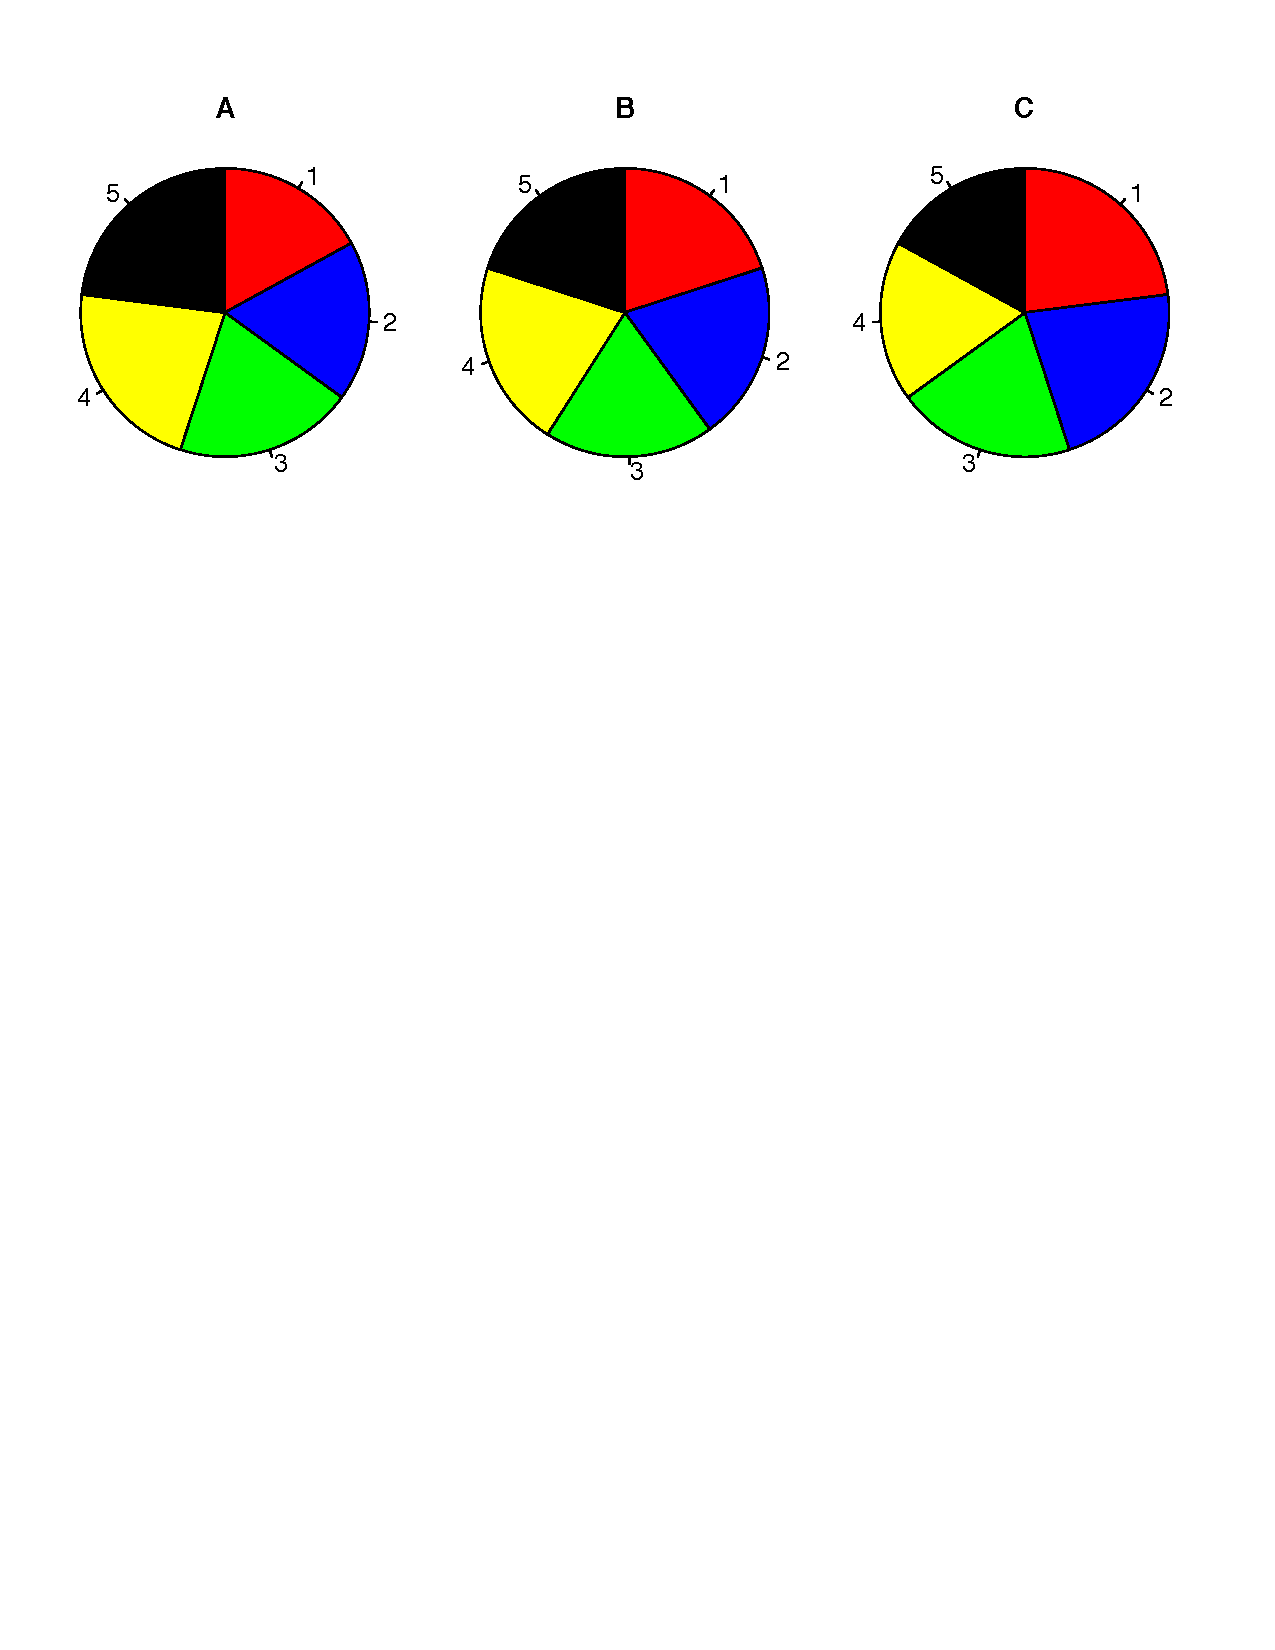
\includegraphics[width=0.9\textwidth]{piecharts-pies}
\end{center}

\begin{solution}
This is much easier if we have bar charts instead:
\begin{center}
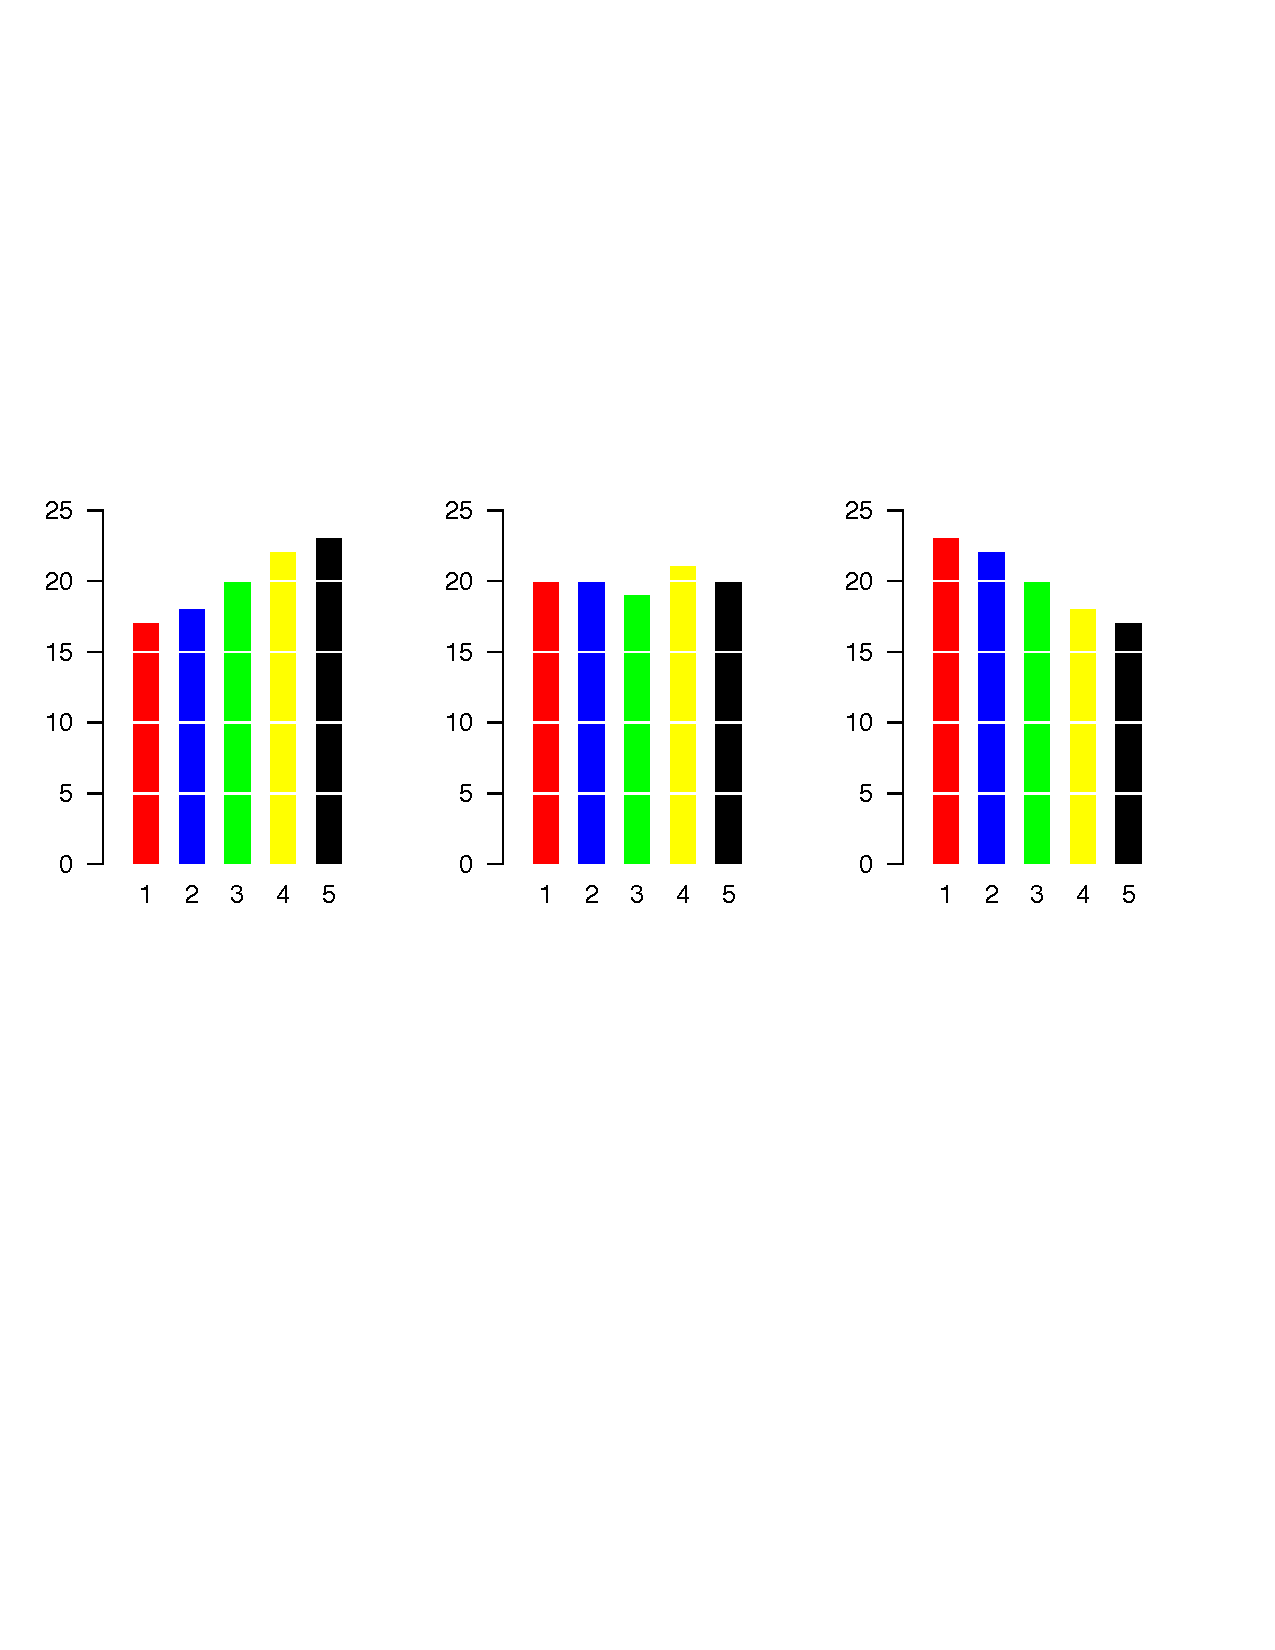
\includegraphics[width=0.9\textwidth]{piecharts-bars}
\end{center}
The relative ordering of the categories is obvious.  The takeaway here is that
you should never use a pie chart; a bar chart conveys the same information,
and it is much easier to read.
\end{solution}



\question List two methods to describe the reported undergraduate majors of
the class survey respondents.

\begin{solution}
Frequency table; bar chart.
\end{solution}
\vspace{\stretch{1}}


\question Draw what you think the bar chart for the birth months of the survey
respondents will look like.

\begin{solution}
\end{solution}
\vspace{\stretch{1}}


%\ifprintanswers\else\newpage\fi

\newpage

\fullwidth{\section*{Describing Numerical (Quantitative) Data}} 

\question Draw what you think the histogram for ``Websites Visited per Day'' will look
like.

\begin{solution}
\end{solution}
\vspace{\stretch{1}}

\question Draw what you think the histogram for ``Dinners per Month'' will look
like.

\begin{solution}
\end{solution}
\vspace{\stretch{1}}


\question Draw what you think the histogram for ``Interest in this Class'' will look like.

\begin{solution}
\end{solution}
\vspace{\stretch{1}}



}

\newpage

\fullwidth{\section*{Measures of Central Tendency}}


\question Here are some histograms.  Estimate the mean and median of the data.

\begin{parts}

\part Symmetric and mound-shaped data.
\begin{center}
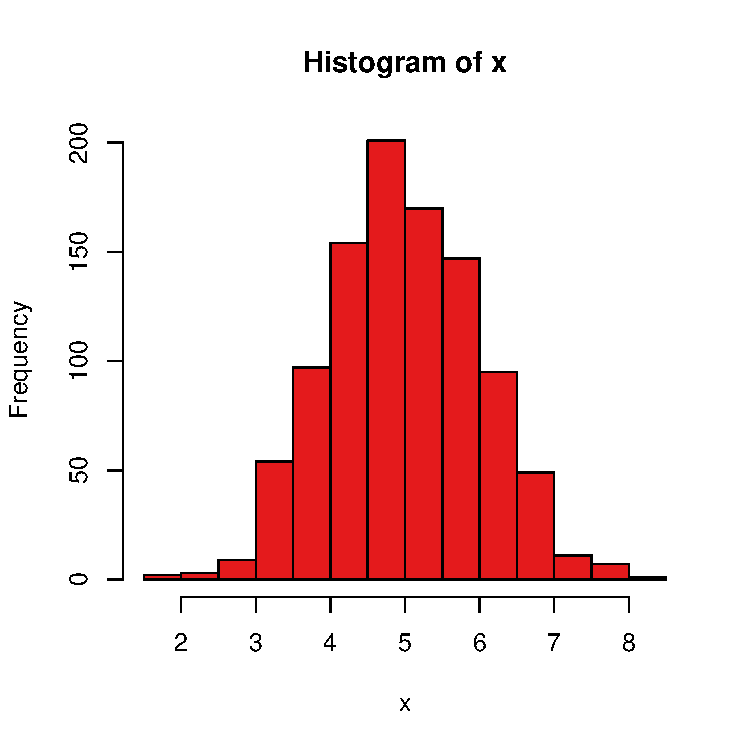
\includegraphics[width=0.35\textwidth]{hist-normal}
\end{center}

\begin{solution}
The median (solid) is roughly in the sample place as the mean (dashed).
\begin{center}
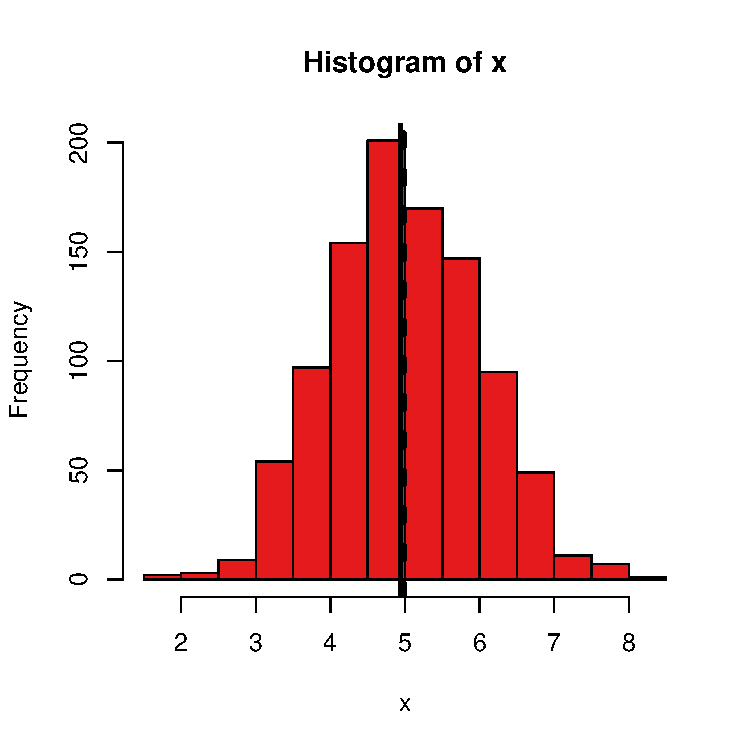
\includegraphics[width=0.35\textwidth]{hist-meanmed-normal}
\end{center}
\end{solution}

%\newpage


\part Skewed data.
\begin{center}
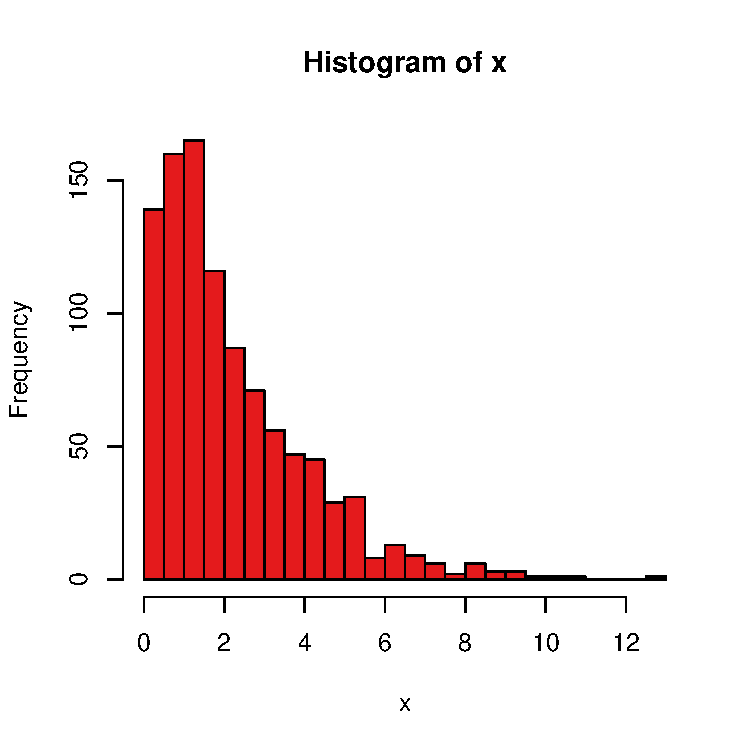
\includegraphics[width=0.35\textwidth]{hist-skew}
\end{center}

\begin{solution}
The mean is pulled to the right by the long tail.
\begin{center}
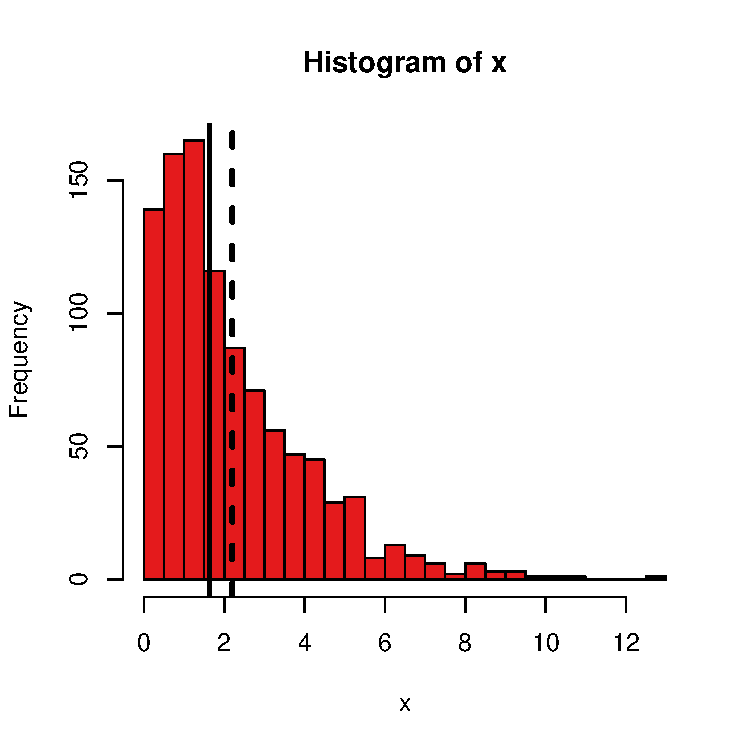
\includegraphics[width=0.35\textwidth]{hist-meanmed-skew}
\end{center}
\end{solution}



\part Bimodal data.
\begin{center}
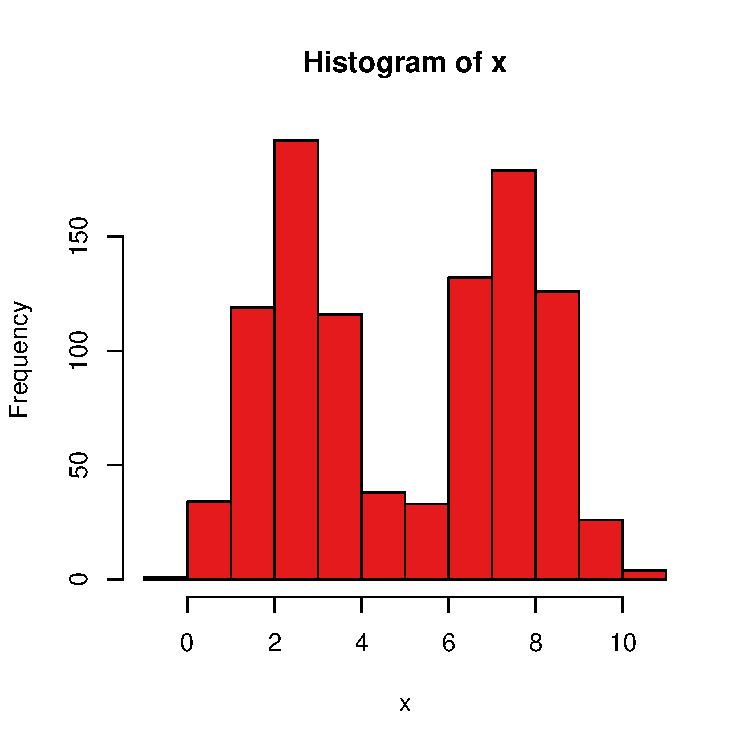
\includegraphics[width=0.35\textwidth]{hist-bimodal}
\end{center}

\begin{solution}
The median and the mean are roughly in the center.  Note that neither number
conveys much information about the distribution.
\begin{center}
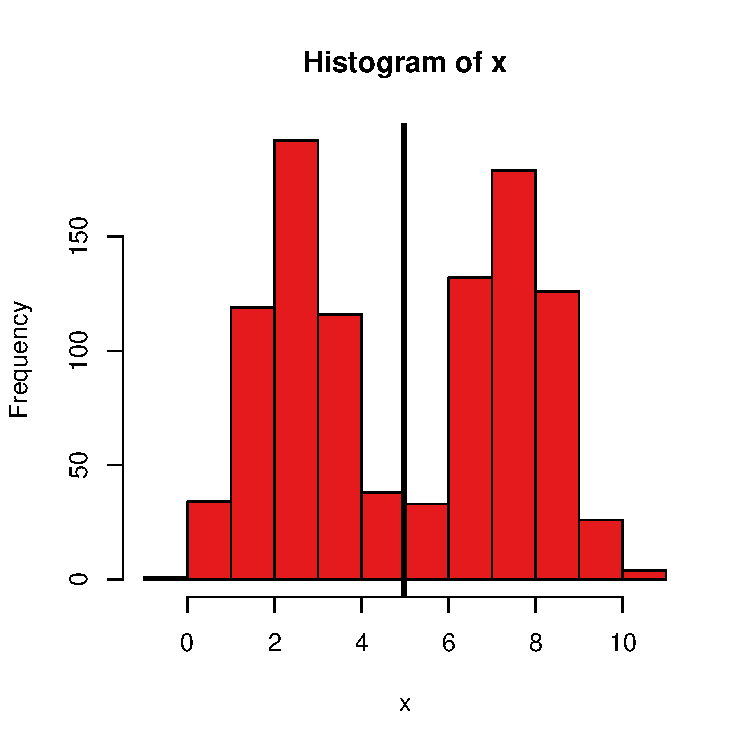
\includegraphics[width=0.35\textwidth]{hist-meanmed-bimodal}
\end{center}
\end{solution}


\end{parts}
\newpage

\question For the examples (a)--(c) of the previous problem, which is
appropriate, the mean or the median?

\begin{solution}
  This depends on context. If we care about ``average'' behavior, then mean is
  typically more appropriate; if we care about ``typical'' behavior, then
  median is typically more appropriate.

(a) Both are appropriate; (b) the median is more appropriate for ``typical''
behavior; mean is more appropriate for ``average'' behavior; (c) mean is
appropriate for ``average''; median is not appropriate.
\end{solution}
%\vspace{\stretch{1}}



%\clearpage

\newpage
\fullwidth{\section*{Standard Deviation and The Empirical Rule}}


\question Forty-three respondents to a Stern MBA class survey reported their GMAT
scores.  The mean score was 710, and the standard deviation was 35.  What can
you say about the range of scores reported?  Assume that the distribution of
reported scores is symmetric and mound-shaped.

\begin{solution}
We can use the empirical rule to make the following statements:
\begin{itemize}
  \item For approximately 68\% respondents, reported score is between 675 and
    745.
  \item For approximately 95\% respondents, reported score is between 640 and
    780.
  \item For approximately 99.7\% respondents, reported score is between 605 and
    815.
\end{itemize}
(For the last interval, it is ok to say ``between 605 and 800,'' since it is
impossible to score above 800.)
In fact the true percentages in those intervals are 67\%, 93\%, and 100\%.
When the distribution of the data is symmetric and mound-shaped, the
predictions from the empirical rule are usually only accurate for the 68\% and
95\% intervals.
\end{solution}


%\question Over the last 50 years, a certain mutual fund has a mean annual
%return of 5\%, with a standard deviation of 2\%.  What can you say about the
%typical performance of the fund?  Assume that the distribution of the annual
%returns is symmetric and mound-shaped.
%
%\begin{solution}
%We can use the empirical rule to make the following statements:
%\begin{itemize}
%  \item 68\% of the time, the return for the fund is between 3\% and 7\%.
%  \item 95\% of the time, the return for the fund is between 1\% and 9\%.
%  \item 99.7\% of the time, the return for the fund is between -1\% and 11\%.
%\end{itemize}
%\end{solution}

\vspace{\stretch{1.5}}


\question Forty-seven respondents from a Stern MBA class survey reported their
expected starting salaries.  The mean reported expected starting salary was
$\$120K$ and the standard deviation was $\$25K$.

\begin{parts}

\part Complete the following statement with appropriate values for $X$ and $Y$:
``Approximately 95\% of the survey respondents have expected starting
salaries between $X$ and $Y$.''

\begin{solution}
$X = 120 - 2 \times 25 = 70$; $Y = 120 + 2 \times 25 = 170$.
\end{solution}

%\begin{solution}
%$X = 3.5 - 2 \cdot 0.3 = 2.9$; $Y = 3.5 + 2 \cdot 0.3 = 4.1$.
%There are no A+ grades at NYU, so the highest possible GPA is 4.0; in light of
%this, we could use $Y = 4.0$ instead of $Y = 4.1$.
%\end{solution}

\vspace{\stretch{1}}

\part What assumptions do you need to make for the statement in (a) to be
correct?  Do you think these assumptions are plausible?  How could you check
this?

\begin{solution}
That the distribution of expected salaries is symmetric and mound-shaped.

We could check this with a histogram.
\end{solution}

\vspace{\stretch{1}}

\part What can we do if the assumptions needed in part (b) are not satisfied?

\begin{solution}
  Sometimes, we can transform the data (e.g., by taking logarithms) to get
  a variable that has a symmetric, mound-shaped histogram. 
\end{solution}


\vspace{\stretch{1}}

\end{parts}

%\question You run a restaurant on Bleecker Street.  Over the past four years,
%the mean number of tables served on Saturday night was 100, and the standard
%deviation was 15 tables.  
%
%\begin{parts}
%
%\part Complete the following statement with appropriate values for $X$ and $Y$:
%``Approximately 95\% of the time, the table serves between $X$ and $Y$ tables
%on Saturday night.''
%
%\begin{solution}
%$X = 100 - 2 \cdot 15 = 70$; $Y = 100 + 2 \cdot 15 = 130$.
%\end{solution}
%
%\vspace{\stretch{1}}
%
%\part What assumptions do you need to make for the statement in (a) to be
%correct?
%
%\begin{solution}
%That the distribution of the number of tables is symmetric and mound-shaped.
%\end{solution}
%
%\vspace{\stretch{1}}
%
%\end{parts}


\newpage

\fullwidth{\section*{$z$-scores}}

\question Your company has an annual profit of \$60MM with a standard
deviation of \$5MM.  Assume that the distribution of your annual profits is
symmetric and mound-shaped.

\begin{parts}

\part Would it be unusual for your company to have an annual profit of \$52MM?

\begin{solution}
No; 95\% of the time, profits are between \$50MM and \$70MM.
\end{solution}

\vspace{\stretch{1}}

\part Would it be unusual for your company to have an annual profit of \$83MM?

\begin{solution}
Yes; this would happen less than 99.7\% of the time.
\end{solution}

\vspace{\stretch{1}}

\end{parts}


\question Forty-seven respondents from a Stern MBA class survey reported their
expected starting salaries.  The histogram of these responses was
approximately bell-shaped.  The mean and standard deviation (in
\$1K$/$year) was was $\bar x = 120$ and $s = 25$.
How many standard deviations above or below the mean are
the following values?

\begin{parts}

\part A starting salary of \$200K.

\begin{solution}
Let $x_1 = 200$ and
let $z_1$ be the number of standard deviations above of below the mean.  Then,
\[
  x_1 = \bar x + s z_1,
\]
so
\[
  z_1 = \frac{x_1 - \bar x}{s} = \frac{200 - 120}{25} = 3.2.
\]
Thus, $x_1$ is $3.2$ standard deviations above the mean.
\end{solution}

\vspace{\stretch{1}}

\part A starting salary of \$100K.

\begin{solution}
Let $x_2 = 100$.  Then,
\[
  z_2 = \frac{x_2 - \bar x}{s} = \frac{100 - 120}{25} = -0.8.
\]
Thus, $x_2$ is $0.8$ standard deviations below the mean.
\end{solution}

\vspace{\stretch{1}}

\part A starting salary of \$170K.

\begin{solution}
Let $x_3 = 170$.  Then,
\[
  z_3 = \frac{x_3 - \bar x}{s} = \frac{170 - 120}{25} = 2.
\]
Thus, $x_3$ is $2$ standard deviations above the mean.
\end{solution}

\vspace{\stretch{1}}

\end{parts}

\question In the previous problem, which of the values are unusual?

\begin{solution}
The value $x_1 = 200$ is unusual, since this is $3.2$ standard deviations
away from the mean.  Typical values are within 2 or 3 standard deviations of
the mean (here, ``typical'' means 95\% or 99.7\% of the time).
\end{solution}

\vspace{\stretch{1}}

% \newpage
% 
% \fullwidth{\section*{Boxplots}}
% 
% 
% \question Here are the 23 reported answers to the question ``How many times do
% you go out to dinner in a typical month'' for the female respondents.
% The quartiles are shown in bold.  Make a boxplot of the data.
% \begin{center}
%   2, 2, 3, 4, 4.5,  5,  5,  6,  6,  6,  7, \textbf{7.5},
%   8, 8, 8, 8,   8, 10, 10, 10, 10, 15, 25
% \end{center}
% 
% \vspace{14.5\baselineskip}
% 
% \begin{tikzpicture}[scale=.15]
% \draw (0,0) -- (100, 0);
% \foreach \x in {0,2,...,30}
%   \draw (\x * 3.333cm, 1cm) -- (\x * 3.333cm, -1cm) node[anchor=north] {$\x$};
% \end{tikzpicture}
% 
% 
% \question Here are the answers for the 30 male survey respondents.
% The middle values are shown in bold.  Make a boxplot of the data.
% \begin{center}
%   0.5, 2, 3,   4,   4, 4, 4, 4,  4,  4,  4,  4,  5,    5, \textbf{6},
%   \textbf{6}, 6, 7, 7.5, 7.5, 8, 8, 9, 10, 10, 10, 12, 13, 13.5, 15
% \end{center}
% 
% 
% 
% \vspace{14.5\baselineskip}
% 
% \begin{tikzpicture}[scale=.15]
% \draw (0,0) -- (100, 0);
% \foreach \x in {0,2,...,30}
%   \draw (\x * 3.333cm, 1cm) -- (\x * 3.333cm, -1cm) node[anchor=north] {$\x$};
% \end{tikzpicture}
% 
% 
% 
% \vspace{\stretch{1}}


\end{questions}

\end{document}

